\documentclass[tikz,border=2pt]{standalone}

\usepackage{pgfplots}
\pgfplotsset{compat=1.18}

\begin{document}
	
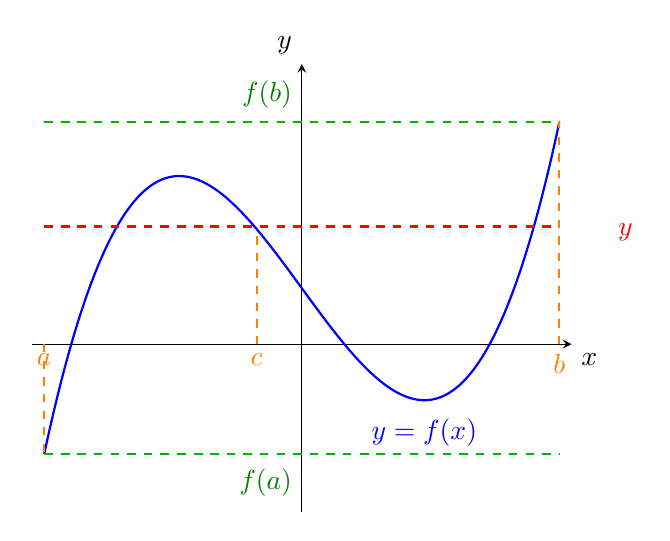
\begin{tikzpicture}
	\begin{axis}[
		axis lines=middle,
		xmin=-2.2, xmax=2.2,
		ymin=-3, ymax=5,
		xtick=\empty, ytick=\empty,
		xlabel={$x$},
		ylabel={$y$},
		xlabel style={below right},
		ylabel style={above left},
		domain=-2.1:2.1,
		samples=200,
		smooth,
		clip=false
		]
		% 绘制函数曲线
		\addplot[thick, blue] {x^3 - 3*x + 1};
		
		% f(a) 和 f(b) 的水平线(绿色)
		\addplot[dashed, green!70!black, thick] coordinates {(-2.1,{(2.1)^3 - 3*(2.1) + 1}) (2.1,{(2.1)^3 - 3*(2.1) + 1})};
		\addplot[dashed, green!70!black, thick] coordinates {( -2.1,{(-2.1)^3 - 3*(-2.1) + 1}) (2.1,{(-2.1)^3 - 3*(-2.1) + 1})}; 
		
		% 红色水平线 y = u
		\addplot[dashed, red, thick] coordinates {(-2.1,2.1) (2.1,2.1)};
		
		% 垂直虚线 a, b, c
		\draw[dashed, orange, thick] (axis cs:-2.1,0) -- (axis cs:-2.1,{(-2.1)^3 - 3*(-2.1) + 1});
		\draw[dashed, orange, thick] (axis cs:2.1,0) -- (axis cs:2.1,{(2.1)^3 - 3*(2.1) + 1});
		\draw[dashed, orange, thick] (axis cs:-0.368,0) -- (axis cs:-0.368,2);
		
		% 标注 f(a), f(b), u
		\node[left, green!50!black] at (axis cs:0,{(-2.1)^3 - 3*(-2.1) + 0.5}) {$f(a)$};
		\node[left, green!50!black] at (axis cs:0,{(2.1)^3 - 3*(2.1) + 1.5}) {$f(b)$};
		\node[right, red] at (axis cs:2.5,2) {$y$};
		
		% 标注 a, b, c
		\node[below, orange] at (axis cs:-2.1,0) {$a$};
		\node[below, orange] at (axis cs:2.1,0) {$b$};
		\node[below, orange] at (axis cs:-0.368,0) {$c$};
		
		% 标注函数
		\node[above, blue] at (axis cs:1,{-2}) {$y=f(x)$};
		
	\end{axis}
\end{tikzpicture}
	
\end{document}